\documentclass[10pt,a4paper]{article}
\usepackage[utf8]{inputenc}
\usepackage[T1]{fontenc}
\usepackage[french]{babel}
\usepackage{hyperref}
\usepackage{geometry}
\geometry{a4paper,margin=10mm,footskip=0mm}
%\setlength\leftmargin{2cm}
%\setlength\rightmargin{2cm}
\fontfamily{ppl}
\usepackage{graphicx}
\setlength\parindent{0pt}
\pagenumbering{gobble}
\frenchbsetup{StandardLists=true} % à inclure si on utilise \usepackage[french]{babel}
%\usepackage{enumitem}
\usepackage{amssymb}

\usepackage{soul}
\usepackage[svgnames]{xcolor}
\sethlcolor{LightYellow}
\newcommand{\grisclair}[1]{\colorbox{LightGray}{#1}}
\newcommand{\rosepale}[1]{\colorbox{BlanchedAlmond}{#1}}
\newcommand{\bleupale}[1]{\colorbox{AliceBlue}{#1}}

\title{\bfseries{SoCo : Création de formulaires d'inscription}}
%\author{Odile Bénassy}
\author{}
\date{}

\begin{document}
\pagestyle{empty}


\maketitle

\emph{Toute utilisatrice autorisée peut créer ses propres formulaires SoCo.}

\emph{À l'Université Paris Sud, il suffit pour cela de posséder un compte sur l'annuaire Adonis.}

\small{\emph{NB: Il est d'un usage de plus en plus répandu d'éviter de privilégier un genre plutôt qu'un autre. Toutefois, nous tenons à préserver la qualité de la langue. En conséquence, pour le présent document, nous adoptons la convention suivante : nous parlons d'un utilisateur - qui peut être aussi bien une utilisatrice bien évidemment - et d'une organisatrice - qui, de même, pourrait être aussi bien un organisateur.}}

\section*{\rosepale{\emph{Création d'un formulaire}}}

\begin{itemize}
  \item Une fois sur le service, identifiez-vous et pénétrez dans l'\emph{espace réservé} (\url{https://soco.jm.u-psud.fr/suivi})
  \item Vous arrivez sur la page d'index du \emph{suivi}, qui reprend la liste de vos colloques en cours (formulaires déjà créés, s'il y en a)
  \item En bas de cette page, cliquez sur \emph{Créer un formulaire d'inscription}
  \item Renseignez : titre, sous-titre, date, date de fin (cas événement sur plus d'un jour), lieu, dates d'ouverture et de clôture des inscriptions
    \item Certains incompatibilités déclenchent une petite alerte : si la date de clôture des inscriptions se trouvait antérieure à la date d'ouverture des inscriptions ; ou encore postérieure à la date de l'événement ; ou si la date de fin de l'événement était antérieure à sa date de début
  \item Si vous le souhaitez, vous pouvez rédiger une question concernant la fréquentation d'un cocktail ou repas ; vous êtes tout à fait libre de la rédaction de cette question
  \item NB : En réalité, il est possible d'ajouter autant de questions supplémentaires que vous le souhaitez $\longrightarrow$ adressez-vous à l'administrateur

\end{itemize}

\begin{figure}[h]
  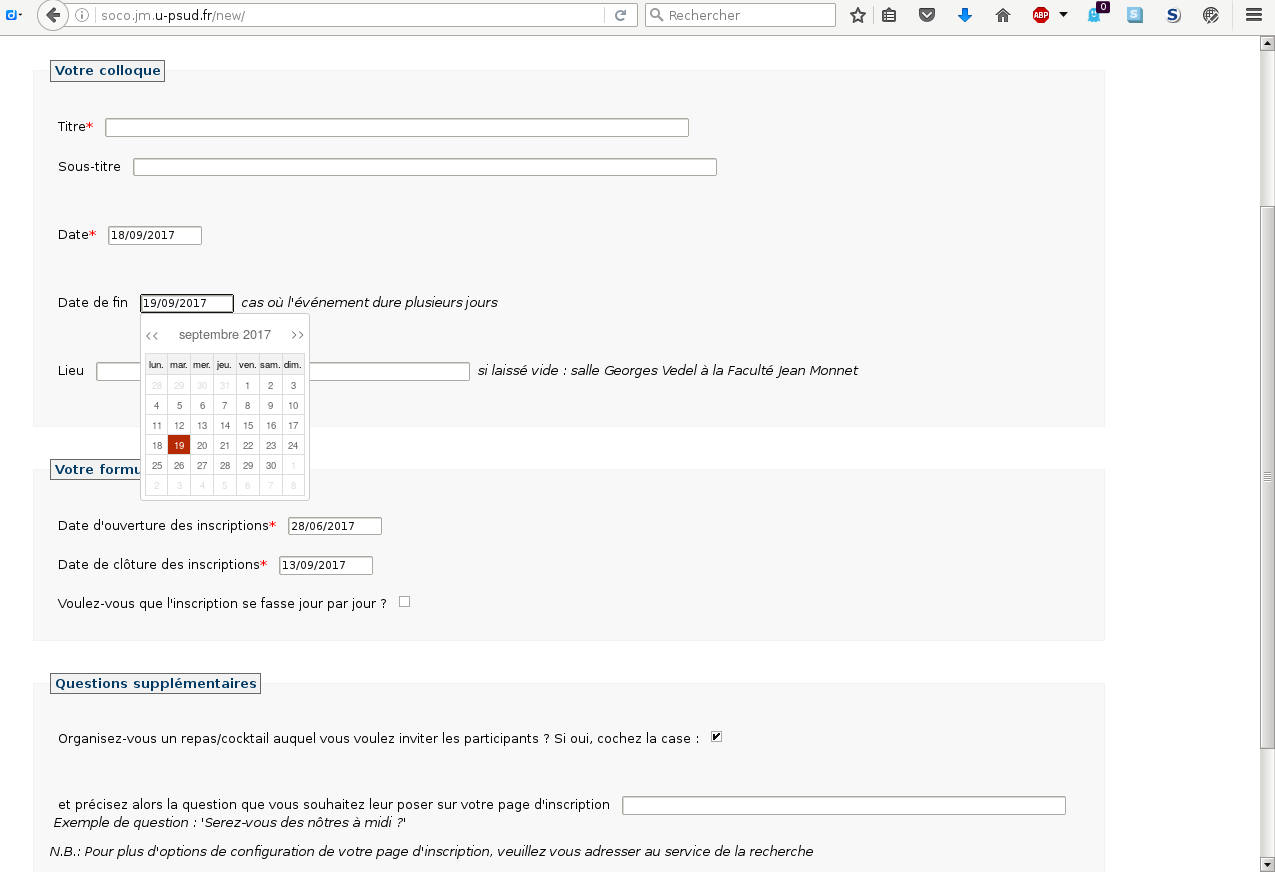
\includegraphics[width=500px]{images/creation-formulaire}
\end{figure}

\section*{\rosepale{\emph{Questions supplémentaires}}}

NB : Il est possible d'ajouter autant de questions supplémentaires que vous le souhaitez $\longrightarrow$ adressez-vous à l'administrateur

Ces questions sont alors affichées sur le formulaire, en bas, à la suite des champs précédents.

\newpage
\section*{\rosepale{\emph{Modification de la date de clôture}}}

\section*{\rosepale{\emph{Visualisation des inscrits}}}

\section*{\rosepale{\emph{Documents à télécharger}}}

\section*{\rosepale{\emph{Export}}}

\section*{\rosepale{\emph{Améliorations prévues}}}

Les améliorations suivantes sont en cours de développement :

\begin{itemize}
\item Formulaire d'inscription spécifique pour les intervenants : jour et heure d'arrivée, frais à rembourser, souhaits hôtellerie...

\end{itemize}

\fcolorbox{Black}{LightGray}{%
  \minipage[t]{\dimexpr0.9\linewidth-2\fboxsep-2\fboxrule\relax}
  \emph{Le logiciel SoCo a été réalisé, à l'UFR Jean Monnet de l'Université Paris Sud, par Odile Bénassy, responsable du service des systèmes d'information, en collaboration avec les responsables du service de la recherche du service de la communication. Ce logiciel prend la suite d'un autre, réalisé en 2007 par la même personne.}
  \endminipage}\hfill

%\fcolorbox{White}{White}{Fertig!}

\end{document}
